\section{Flights in time and along their route}\label{sec:flights}

Does a real flight follow the crests as straight as a ball at constant speed, and what changes when its exponent is measured
along the route instead of in time? We compare three curves for the paragliders of each massif (Section~\ref{sec:flcurves}
defines them): the crests, the flights in time and the route of the flights, which is the track in arc length with every
thermal climb replaced by its chord. Figure~\ref{fig:routealpha} gives their local slope $\alpha$, Table~\ref{tab:flh}
their exponent $H$ and Figure~\ref{fig:routemsd} their MSD.

\begin{figure}
\centering
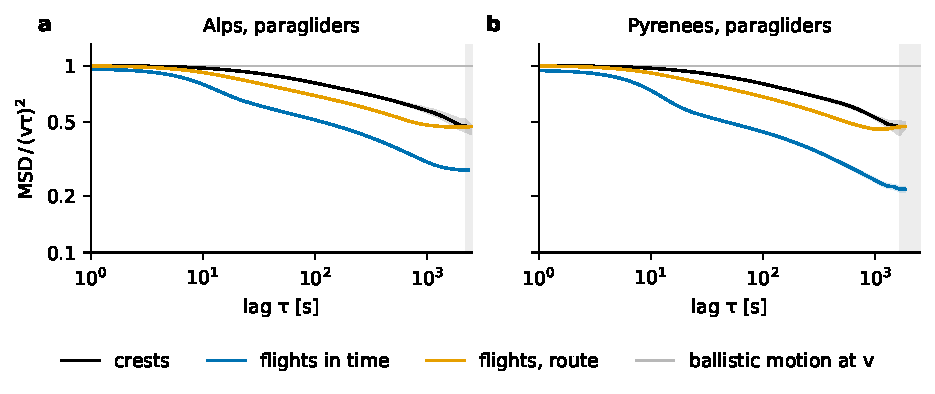
\includegraphics[width=\textwidth]{figures/route_msd}
\caption{The route of the flights stays close to the crests, and the flights in time fall below both. Mean squared
displacement over the ballistic value, $\overline{\delta^2}(\tau)/(v\tau)^2$, of the crests, the route and the flights in time
against the lag $\tau$, for the Alps (\textbf{a}) and the Pyrenees (\textbf{b}) paragliders. Grey line: 1, a ballistic motion at
speed $v$. Bands: 95\% bootstrap intervals; grey zone: beyond the last lag of the fit.}
\label{fig:routemsd}
\end{figure}

In both massifs the route is a little below the crests and the flights in time are well below the route
(Table~\ref{tab:flh}). The curves of $\alpha$ in Figure~\ref{fig:routealpha} show where the flights in time differ from the
route. They leave the ballistic value within seconds, fall to a minimum in the first twenty seconds, which is about half a turn of
a circle, and recover part of the way. The route has no such minimum. Towards the last lag of the fit the curves of the flights
rise, because only the longest flights reach these lags and they are the straightest; the fit stops there.

The order is the same on fixed windows of arc length (Table~\ref{tab:flwindows}, Appendix~\ref{app:checks}). Fitting the flights
in time from 10~s gives a higher exponent, for the same reason that $\alpha$ rises at long lags, so it is not the number compared
with the crests. The cleaning of the tracks does not change the exponent within the interval of the sample that checks it.

\paragraph{What we keep.} Along the route a paraglider flight is about as straight as the crests. In time the exponent is lower
because of the circles. How the route is travelled in time is the subject of the companion document in the folder
\code{intermittency/}.
